\documentclass[varwidth=true, border=2pt]{standalone}

\usepackage{pgfplots}
\usepackage{tikz}

\begin{document}
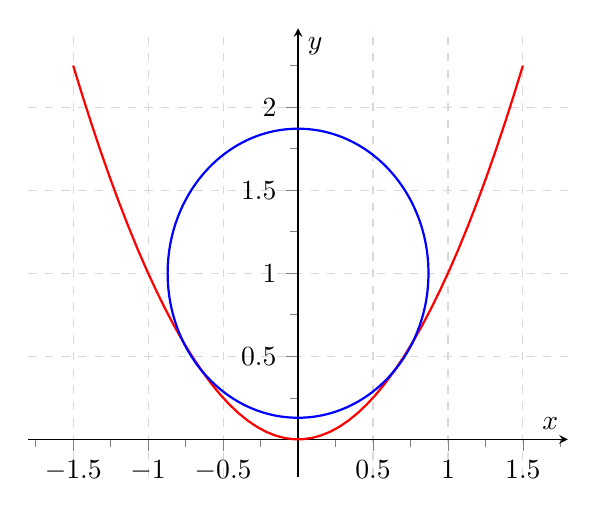
\begin{tikzpicture}
    \begin{axis}[
        legend pos=south west,
        axis x line=middle,
        axis y line=middle,
        grid = major,
        %width=9cm,
        %height=9cm,
        grid style={dashed, gray!30},
        xmin=-1.5,     % start the diagram at this x-coordinate
        xmax= 1.5,    % end   the diagram at this x-coordinate
        %ymin=-0.25,     % start the diagram at this y-coordinate
        %ymax= 2.25,   % end   the diagram at this y-coordinate
        axis background/.style={fill=white},
        xlabel=$x$,
        ylabel=$y$,
        %xticklabels={-2,-1.6,...,7},
        %yticklabels={-8,-7,...,8},
        tick align=outside,
        minor tick num=-3,
        enlargelimits=true,
        tension=0.08]
      \addplot[domain=-1.5:1.5, red, thick,samples=50] {x*x};
	\draw[blue, thick] \pgfextra{
	  \pgfpathellipse{\pgfplotspointaxisxy{0}{1}}
		{\pgfplotspointaxisdirectionxy{0.87}{0}}
		{\pgfplotspointaxisdirectionxy{0}{0.87}}
	  % see also the documentation of
	  % 'axis direction cs' which
	  % allows a simpler way to draw this ellipse
	};
    \end{axis}
\end{tikzpicture}
\end{document}
